%%%%%%%%%%%%%%%%%%%%%%%%%%%%%%%%%%%%%%%%%%%%%%%%%%%%%%%%%%%%%%%%%%%%%%%%%%%%%%%%%%%%%%
% Modelo de relatório de Disciplina de MLP a partir da
% classe latex iiufrgs disponivel em http://github.com/schnorr/iiufrgs
%%%%%%%%%%%%%%%%%%%%%%%%%%%%%%%%%%%%%%%%%%%%%%%%%%%%%%%%%%%%%%%%%%%%%%%%%%%%%%%%%%%%%%

%%%%%%%%%%%%%%%%%%%%%%%%%%%%%%%%%%%%%%%%%%%%%%%%%%%%%%%%%%%%%%%%%%%%%%%%%%%%%%%%%%%%%%
% Definição do tipo / classe de documento e estilo usado
%%%%%%%%%%%%%%%%%%%%%%%%%%%%%%%%%%%%%%%%%%%%%%%%%%%%%%%%%%%%%%%%%%%%%%%%%%%%%%%%%%%%%%
%
\documentclass[rel_mlp]{iiufrgs}

%%%%%%%%%%%%%%%%%%%%%%%%%%%%%%%%%%%%%%%%%%%%%%%%%%%%%%%%%%%%%%%%%%%%%%%%%%%%%%%%%%%%%%
% Importação de pacotes
%%%%%%%%%%%%%%%%%%%%%%%%%%%%%%%%%%%%%%%%%%%%%%%%%%%%%%%%%%%%%%%%%%%%%%%%%%%%%%%%%%%%%%
% (a A seguir podem ser importados os pacotes necessários para o documento, de acordo 
% com a necessidade)
%
\usepackage{float}
\usepackage[brazilian]{babel}	    % para texto escrito em pt-br
\usepackage[utf8]{inputenc}         % pacote para acentuação
\usepackage{graphicx}         	    % pacote para importar figuras
\usepackage[T1]{fontenc}            % pacote para conj. de caracteres correto
\usepackage{times}                  % pacote para usar fonte Adobe Times
\usepackage{enumerate}              % para lista de itens com letras
\usepackage{breakcites}
\usepackage{titlesec}
\usepackage{enumitem}
\usepackage{titletoc}               
\usepackage{listings}			    % para listagens de código-fonte
\usepackage{mathptmx}               % p/ usar fonte Adobe Times nas formulas matematicas
\usepackage{url}                    % para formatar URLs
%\usepackage{color}				    % para imagens e outras coisas coloridas
%\usepackage{fixltx2e}              % para subscript
%\usepackage{amsmath}               % para \epsilon e matemática
%\usepackage{amsfonts}
%\usepackage{setspace}			    % para mudar espaçamento dos parágrafos
%\usepackage[table,xcdraw]{xcolor}  % para tabelas coloridas
%\usepackage{longtable}             % para tabelas compridas (mais de uma página)
%\usepackage{float}
%\usepackage{booktabs}
%\usepackage{tabularx}
%\usepackage[breaklinks]{hyperref}

\usepackage[alf,abnt-emphasize=bf]{abntex2cite}	% pacote para usar citações abnt

%%%%%%%%%%%%%%%%%%%%%%%%%%%%%%%%%%%%%%%%%%%%%%%%%%%%%%%%%%%%%%%%%%%%%%%%%%%%%%%%%%%%%%
% Macros, ajustes e definições
%%%%%%%%%%%%%%%%%%%%%%%%%%%%%%%%%%%%%%%%%%%%%%%%%%%%%%%%%%%%%%%%%%%%%%%%%%%%%%%%%%%%%%
%

% define estilo de parágrafo para citação longa direta:
\newenvironment{citacao}{
    %\singlespacing
    %\footnotesize
    \small
    \begin{list}{}{
        \setlength{\leftmargin}{4.0cm}
        \setstretch{1}
        \setlength{\topsep}{1.2cm}
        \setlength{\listparindent}{\parindent}
    }
    \item[]}{\end{list}
}

% adiciona a fonte em figuras e tabelas
\newcommand{\fonte}[1]{\\Fonte: {#1}}

% Ative o seguinte caso alguma nota de rodapé fique muito longa e quebre entre múltiplas
% páginas
%\interfootnotelinepenalty=10000

%%%%%%%%%%%%%%%%%%%%%%%%%%%%%%%%%%%%%%%%%%%%%%%%%%%%%%%%%%%%%%%%%%%%%%%%%%%%%%%%%%%%%%
% Informações gerais                                   
%%%%%%%%%%%%%%%%%%%%%%%%%%%%%%%%%%%%%%%%%%%%%%%%%%%%%%%%%%%%%%%%%%%%%%%%%%%%%%%%%%%%%%

% título
\title{Grupo Equipe 7 \\ Projeto Space Invaders Utilizando Lua} 

% autor
\author{Fischer Comerlato}{Felipe} % {sobrenome}{nome}
\author{Eich}{Leonardo} % {sobrenome}{nome} 

% Professor orientador da disciplina
\advisor[Prof.~Dr.]{Mello Schnorr}{Lucas}

% Nome do(s) curso(s):
\course{Curso de Graduação em Ciência da Computa{\c{c}}{\~a}o e Engenharia de Computação}

% local da realização do trabalho 
\location{Porto Alegre}{RS} 

% data da entrega do trabalho (mês e ano)
\date{09}{2018}


% Palavras chave
\keyword{Palavra-chave1}
\keyword{Palavra-chave2}
\keyword{Palavra-chave3}


%%%%%%%%%%%%%%%%%%%%%%%%%%%%%%%%%%%%%%%%%%%%%%%%%%%%%%%%%%%%%%%%%%%%%%%%%%%%%%%%%%%%%%
% Início do documento e elementos pré-textuais
%%%%%%%%%%%%%%%%%%%%%%%%%%%%%%%%%%%%%%%%%%%%%%%%%%%%%%%%%%%%%%%%%%%%%%%%%%%%%%%%%%%%%%

% Declara início do documento
\begin{document}

% inclui folha de rosto 
\maketitle      

\selectlanguage{brazilian}

% Sumario
\tableofcontents



%%%%%%%%%%%%%%%%%%%%%%%%%%%%%%%%%%%%%%%%%%%%%%%%%%%%%%%%%%%%%%%%%%%%%%%%%%%%%%%%%%%%%
% Aqui comeca o texto propriamente dito
%%%%%%%%%%%%%%%%%%%%%%%%%%%%%%%%%%%%%%%%%%%%%%%%%%%%%%%%%%%%%%%%%%%%%%%%%%%%%%%%%%%%%

%espaçamento entre parágrafos
%\setlength{\parskip}{6 pt}

\selectlanguage{brazilian}



%%%%%%%%%%%%%%%%%%%%%%%%%%%%%%%%%%%%%%%%%%%%%%%%%%%%%%%%%%%%%%%%%%%%%%%%%%%%%%%%%%%%%
% Introdução
%
\chapter{Introdução} \label{intro}

Este trabalho tem como objetivo o estudo de uma linguagem de programação moderna com características híbridas contextualizando os conceitos vistos em aula ao longo do semestre e, por fim, analisar e avaliar diferentes linguagens de programação, seguindo os critérios vistos em aula.

A tarefa principal do trabalho consiste em experimentar e comparar as características e funcionalidades orientadas a objeto e funcionais da linguagem de programação escolhida. De posse de uma linguagem, é necessário escolher um problema a ser solucionado com ela. O problema será, então, implementado duas vezes na mesma linguagem: uma delas usando somente Orientação a Objetos e a outra usando somente características funcionais.

O desenvolvimento do trabalho encontra-se em \url{https://github.com/felipefcomerlato/mlp_equipe7_2018-2}.


\chapter{O Problema}
O problema a ser resolvido neste trabalho é o desenvolvimento do jogo Space Invaders. O jogo expõe o jogador como uma espaçonave que deve destruir as espaçonaves inimigas que querem invadir o planeta do jogador. Na medida que elas avançam na tela (de cima para baixo), o jogador guia sua espaçonave horizontalmente e efetua disparos para destruir todas as ondas de inimigos que se seguem, como visto na Figura \ref{fig:figura1}


\begin{figure}[H]
     \centering
     \caption{Tela do jogo Space Invaders}
     \fbox{
         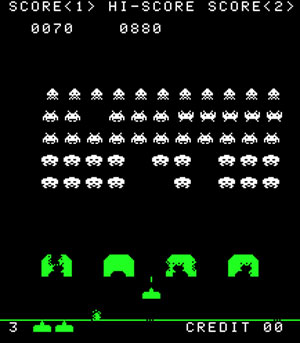
\includegraphics[width=5cm, keepaspectratio]{images/space-invaders-screen.jpg}
     }
     \label{fig:figura1}
     \fonte{http://g1.globo.com/tecnologia/noticia/2011/10/homem-quebra-recorde-mundial-em-space-invaders-jogo-de-1978.html}
 \end{figure}


\chapter{Visão Geral da Linguagem}

A linguagem escolhida para o trabalho foi extbf{Lua}. Lua é uma linguagem de script de multiparadigma, pequena, reflexiva e leve, projetada para expandir aplicações em geral, por ser uma linguagem extensível (que une partes de um programa feitas em mais de uma linguagem), para prototipagem e para ser embarcada em softwares complexos, como jogos. Assemelha-se com Python, Ruby e Icon, entre outras.

Lua foi criada por um time de desenvolvedores do Tecgraf da PUC-Rio, a princípio, para ser usada em um projeto da Petrobras. Devido à sua eficiência, clareza e facilidade de aprendizado, passou a ser usada em diversos ramos da programação, como no desenvolvimento de jogos (a Blizzard Entertainment, por exemplo, usou a linguagem no jogo World of Warcraft), controle de robôs, processamento de texto, etc. Também é frequentemente usada como uma linguagem de propósito geral.

Uma das características principais da linguagem é sua única estrutura de dados: tabelas - que podem ser usadas para representar arrays comuns, sequências, tabelas de símbolos, conjuntos, registros, grafos, árvores, etc.

Lua é uma linguagem distribuída e pode ser compilada em qualquer plataforma que tenha um compilador da linguagem C. Lua pode ser executada em ambientes Unix e Windows, em dispositivos móveis (Android, iOS, Windows Phone, etc), em microprocessadores embarcados e etc.

Incluir Lua numa aplicação não aumenta quase nada o seu tamanho. O pacote de Lua 5.3.5, contendo o código fonte e a documentação, ocupa 297K comprimido e 1.2M descompactado. O fonte contém cerca de 24000 linhas de C. No Linux de 64 bits, o interpretador Lua contendo todas as bibliotecas padrões de Lua ocupa 247K e a biblioteca Lua ocupa 421K \cite{AboutLua}.

Lua possui interpretação dinâmica, ou seja, a linguagem é capaz de executar trechos de código criados dinamicamente, no mesmo ambiente de execução do programa. Como exemplos dessa facilidade temos a função \textit{loadstring} em Lua e a função \textit{eval} em Scheme/Lisp e Perl. Lua possui também tipagem dinâmica forte, ou seja, a linguagem faz verificação de tipos em tempo de execução do programa. Linguagens com
tipagem dinâmica em geral não possuem declarações de tipos no código e não fazem verificação de tipos em tempo de compilação. Tipagem forte significa que a linguagem jamais aplica uma operação a um tipo incorreto. Além disso, Lua conta com gerência automática de memória dinâmica ("coleta de lixo"), por tanto não precisamos gerenciar memória explicitamente no nosso programa; em especial, não há necessidade de um comando para liberar memória após seu uso \cite{IntroLuaPDF}.



\section{Modelo Funcional}

Lua oferece suporte ao modelo de programação funcional mas nos proporciona algumas dificuldades, como a de copiar tabelas, por exemplo, já que tal estrutura de dados atribuída a uma variável é apenas uma referência. Tal dificuldade contraria uma das principais características do próprio paradigma funcional: a de usar funções puras, criando novas estruturas ao invés de alterar uma estrutura original. Por outro lado, Lua nos permite representar funções anônimas através de blocos de código chamados de trechos, característico no modelo funcional. \cite{ManualLua}

\section{Modelo Orientado a Objetos}

O suporte para a programação no paradigma orientado a objetos utilizando Lua é muito vasto. É possível encontrar inúmeros tutoriais para a solução de diversos problemas na linguagem fazendo uso deste paradigma. Como não vimos diversos pré-requisitos necessários para a implementação deste trabalho, não podemos analisar com mais propriedade o desempenho da linguagem Lua neste modelo de programação.


% ----------------------- %

\chapter{Recursos Funcionais}

\section{Elementos Imutáveis e Funções Puras}

\section{Funções Anônimas}

\section{Currying}

\section{Pattern Matching}

\section{Funções de Ordem Superior}

\section{Funções de Ordem Maior Fornecidas Pela Linguagem}

\section{Funções como Elementos de Primeira Ordem}

\section{Recursão}

% ----------------------- %

\chapter{Recursos de Orientação à Objetos}

\section{Classes}

\section{Encapsulamento e Proteção dos Atributos}

\section{Construtores}

\section{Destrutores}

\section{Espaços de Nomes Diferenciados}

\section{Mecanismos de Herança}

\section{Polimorfismo por Inclusão}

\section{Polimorfismo Paramétrico}

\section{Polimorfismo por Sobrecarga}

\section{Delegates}

\chapter{Conclusão Final}



%%%%%%%%%%%%%%%%%%%%%%%%%%%%%%%%%%%%%%%%%%%%%%%%%%%%%%%%%%%%%%%%%%%%%%%%%%%%%%%%%%%%%



%%%%%%%%%%%%%%%%%%%%%%%%%%%%%%%%%%%%%%%%%%%%%%%%%%%%%%%%%%%%%%%%%%%%%%%%%%%%%%%%%%%
% Referências 
%%%%%%%%%%%%%%%%%%%%%%%%%%%%%%%%%%%%%%%%%%%%%%%%%%%%%%%%%%%%%%%%%%%%%%%%%%%%%%%%%%%
%

%\bibliographystyle{abnt}


\bibliographystyle{abntex2-alf}
%bibliographystyle{plain}
%\bibliographystyle{ieeetr}

\bibliography{biblio} % arquivo que contém as referências (no formato bib). Colocar as suas lá (se tiver dúvida sobre como adicionar novas referências, usar o software JabRef ou Medley)




\end{document}
